\documentclass[journal]{IEEEtran}
\usepackage{epsf,cite,amsmath,amscd,graphics,graphicx,latexsym,multicol,setspace}
\usepackage{amsfonts,amsmath,amssymb,amsthm}
\usepackage{scalefnt}
\newcounter{MYtempeqncnt}
\begin{document}
\title{Audio Event Classification Using Audio Embeddings from the AudioSet Data}

\author{Sajeel Aziz*\\
*skaziz@ryerson.ca\\
Department of Electrical and Computer Engineering\\
Ryerson University, Toronto, Canada.}
\maketitle

\begin{abstract}
The aim of this work is to conceptualize a framework for capturing and classifying audio events using audio embeddings that were processed from YouTube audio data. These embeddings are vectors which represent the most important or distinct features of the audio data which can be used in a downstream model for classification. These features are generated by applying a PCA transform and quantizing the data. Therefore, it is also expected that the model using these embeddings will be less complex than if we use a model directly on the audio data. This is an advantage for classification models that will use these embeddings, as it is similar to transfer learning in that respect, The goal of this work is to explore some of the possibilities that utilizing these embeddings can bring.

\end{abstract}

\section{INTRODUCTION}

Many pieces of literature discuss the different methods that could be used for working with audio data. The methods specifically mentioned are Recurrent Neural Networks(RNNs), Long-Term Short-Term RNNs, using Convolutional Neural Networks(CNN’s) to extract information from 2 dimensional representation of the audio like a spectrogram or melgram, use a combination of CNN’s and LSTM RNNs, or fully connected Neural Networks (NN’s). Using the technique described in this paper and scaling it successfully, a captioning system can be developed in any piece of audio which is preprocessed by the VGGish model. Using a generalized version of this system, we can potentially use the audio that was recorded and identify the scene where the recording was captured as well as segment the different events by time within the recording. An example would be, if there are sounds of many cars in the background, it should know that these are car noises and that the audio was probably recorded on a busy street. The practical applications of this system could be to help people with hearing disabilities get a sense of the different background noises in a video. Another use case could be to help police find out the location of interest based on some audio recording from a telephone call.

\section{PROBLEM STATEMENT}

This paper explores the different possibilities of classifying audio events using pre-processed audio data from the researchers who released the data. First, it will look at how to make single classifications using CNNs and ONNs with different batch-sizes and losses. Next, it will also look at outputting multiple labels. The effectiveness of the different strategies will be evaluated. The ultimate goal of this work is to present a framework that can be generalized to classify audio events and recognize where in a recording they occur, while eventually being able to work as a captioning system in a regular audio clip.

\section{RELATED WORK}

One instance of the research combines some of the labels from the AudioSet data to deal with potential confusion or ambiguity in the classification of the audio by the algorithm. After these label changes, it also had to add a few training examples from the “unbalanced” data from this dataset so that the new labels(speech/no-speech and music/no-music) would get an equal amount of training data. 
The most effective architecture was a combination of 2d Convolution and LSTM RNN’s where first an X number of filters are used to get information from the time and frequency dimensions, then the information is passed to the LSTM layer having an X number of units. Through this method, the time-based information can be kept along with the frequency information \cite{1}.

Another approach called Multiple Instance Learning (MIL) could be applied to the AudioSet data. This architecture treats each audio clip as a “Bag” of instances, where each Bag has short clips within the video called an instance. Then, all the event labels associated with that specific audio clip are assigned to that Bag. This is to indicate that these events are present in that “Bag of Instances”.
A CNN is used for this purpose because a frequency-time spectrogram can be viewed as an image. Another method that this paper proposes is to use a CNN that is trained to produce audio embeddings. Then, the embeddings are used as an input to fully-connected layers, which will use a sigmoid function and max-pooling to classify the audio \cite{2}.

A method has also been proposed to use transfer learning from a model trained on Audioset. This will start with a CNN model which will be transferred to adapt to other datasets for different applications. Two of the applications mentioned in this paper are simple “sound event” classifications and also “acoustic scene” classifications. This method can achieve an 83.5 percent accuracy with a computationally efficient method such as a CNN, while being able to make connections between the sound events and scenes \cite{3}.

Another MIL approach can fundamentally be used using Support Vector Machines (SVMs), or by using NN’s. This can understand the temporal and event-based information of the audio data. This can be done by using applying a method called the Gaussian Mixture Model (GMM) to get the information from longer segments of the videos and shorter versions as well. After the feature extraction from the GMM, they are fed into the Neural Network \cite{4}.

Another method of dealing with the weakly labelled data in audioset is by an architecture which included CNN’s was proposed which can work with audio clips of different durations and can change the instances of the clip. There are also some challenges with noise due to the labels of the weakly labelled data. Some more challenges and suggestions raised were to find data from the web with weak labels and compare it to the audio set so that the models that are built in the future can adapt to the changes in the way the data is labelled \cite{5}.


A survey on the different methods used in machine learning for audio event detection shows more approaches for this task. One of the approaches is to use a Gaussian Mixture Model (GMM), which looks at the means and variances of the features in the audio event, for each event type. These GMM’s will result in output probabilities which will be integrated by time, where the highest probability will be chosen as the correct classification for the event. There are other methods to perform the required task such as Hidden Markov Models, Support Vector Machines, and nonnegative matrix factorization. However, the best method to detect sound events use CNN’s or RNN’s as these can detect both frequency and temporal relationships in the audio data \cite{6}.

A feed forward Deep Neural Network can also classify multiple sound events. This goal can be achieved through the hidden layers of the Deep Neural Network (DNN). This method will use the frequency-based features to recognize the relationship between the frequencies and the sound events. Using multi-label classifications, the goal is to recognize overlapping sounds to have a segmentation of each sound that occurs in the audio recording which can be used in a realistic scenario in the field. For this reason, ways to reduce noise in the output by post-processing the data were investigated, so that the small time-frame of the recordings being analyzed don’t confuse the model with it’s intermittent sounds \cite{7}. 


There are also possibilities to carry out Sound Event Detection and tagging simultaneously. It uses the log mel-band audio to input into the new architecture which consists of a joint CNN and RNN so that there are 2 outputs for the strong and weak labels. We produce the strong labels by repetition of the weak labels in the instances of the audio. Therefore, we can train the outputs using both the strong and weak labels and calculate the losses separately for the 2 outputs. The weak labels will be given more significance during training, but strong labels will be used to output the weak labels during the testing \cite{8}.

There is also an application for automatically discovering noisy objects from videos from a set of weakly labelled data. The model can extract some proposals of the correct location of the object in the image. After this step, the best proposals are by using a voting and matching mechanism. At the end, the results are used as strongly labelled data so that there can be lower level segmentation. This approach can help with audio analysis because audio analysis can also use CNN’s which can find certain signatures in the frequency-time based 2-dimensional data \cite{9}.

The possibility of a time-frequency segmentation architecture to process sound events and their temporal features from weakly labelled data has also been investigated. First, the log-mel spectrogram is used to have a representation of the time and frequencies as a function of the time. There is a segmentation and classification applied using CNN’s. This is done through the result of the convolutional operations that give a mapping of the time-frequency value to the clip segmentation and classification. The final classification is done through a pooling system \cite{10}.



\section{METHOD}

This work uses the AudioSet dataset, which is a dataset of nearly 2 million audioclips with weakly labelled data for different segments of a video. It has approximately 600 identified sounds which can be classified through a machine learning model. The initial processing of the data that is used by this work has been done by the VGGish modules which are released by researchers working on AudioSet \cite{11}. The VGGish modules preprocess the audio data by taking a waveform from a wav file and turning it into  an array output with the shape [number of samples, number of features, number of mel bands]. The frame length for the samples is predefined, so the dimension remains constant. This process is done by taking the number of samples information from the data and converting it into number of frames and window length, thus adding a dimension to the data. The result of this will be a number of frames. Next, a periodic hanning window is made using a cosine function to perform the Fourier analysis later. The frames and the window are multiplied and FFT is performed on them where the result is a 2 dimensional array with the length (FFT length)/2 +1 where FFT  length is 256. Next, a matrix of values is prepared that will be multiplied by the spectrogram value matrix to make the mel-spectrogram which has the dimensions [frames, number of mel bins]. This is done by processing the given signal by using given frequency information and putting them into a matrix. After that, the spectrogram and mel matrix are used for a dot product operation which returns the 2D array of values of the dimension [number of frames, number of mel bins]. Next, the resultant features are divided into frames once again. The post processing step takes this resulting array, applies a pca transformation to it and converts it into an 8-bit range, which makes the vectors between the range [0,255]. Next, the post processed data was written as a tensorflow sequence example where each row corresponds to 96 10 millisecond frames of data, which results to approximately 1 second per row.

 The data downloaded was in the form of these processed vectors of length 128, called audio embeddings, stored in tfrecord format where each group of 128 length vectors represent roughly 1 second of the audio data. The features were recorded by opening the tfrecord files one-by-one in the location of its download, converting the byte values to integers between 0 and 255, then looping through the features to store them in a list. For the purposes of this work, some other context label information was used to isolate 4 of the classes i.e. “Human Speech”, “Animal”, “Music” and “Vehicle”. These labels were stored in another array if they simply satisfy the condition to be present in the list of the multiple labels given to that audio clip, whatever other labels they may have. Also, to avoid complications, it was made sure that there were 10 vectors, representing 10 seconds in the data, or else the data was not used. 

The data was then reshaped by making each 128-length audio embedding vector into a set of 10 vectors, so that it can be used for a 2D Convolutional Neural Network. This way, a heatmap is formed for each sample, where the y-axis will be the time between 1 and 10 seconds, the x-axis will be the index of the vector elements, and the pixel intensity values will be the value of the embedding at that position in time. The aim is for the CNN to recognize features from this heatmap of audio embeddings by running filters through it and be able to classify which category that audio clip belongs to.Another approach that was taken was to take all 10 seconds of the audio embeddings, flatten them into a 1280-length vector and use them as imputs to a fully connected neural network. These approaches will be compared in the results section.

One of the challenges that was faced after this process was that there was mostly just data with the labels “Music” and “speech”, which will hinder the training process for animal and vehicle categories. To solve this issue, the data for animal and vehicle categories was shuffled over and over again until there was enough for proper training. This shuffling was done by switching the vectors’ placement in seconds. For example, if a 128 length embedding vector was representing the 1st second, it was switched with another second which was determined by a random number generated between 0 and 10. The data was then split into training and testing sets by using 60 percent training data and 40 percent for testing.

A more ideal way to deal with this type of a classification problem is to have the ability output multiple labels, since each piece of data technically has multiple labels. This was done in keras by adding multiple losses in the model “compile” function, and multiple labels in the model “fit” function. Effectively a model was created consisting of other models and compile it, then name the output of each model, which will serve as the multiple targets to back-propagate against using a dictionary of losses whose keys are the names of the outputs.

\section{RESULTS}

A few experiments were run using the embedding provided by the VGGish modules. The aim of these experiments were to be able to distiguish 4 classes, namely "Speech", "Animal", "Music" and "Vehicle", out of the dataset where 1 of the 4 were present. The effect of each trial are discussed below


\emph {Architecture of CNNs used:}
\\
\\
Layer 1(2D Convolution): 16 filters, 1x6 kernel, 2 vertical and 2 horizontal strides, ReLu activation\\
Layer 2(Max-pooling):2x2 kernel, 1 vertical stride x 1 horizontal\\
Layer 3(2D Convolution): 32 filters, 1x6 kernel, 1 vertical and 1 horizontal strides, ReLu activation, with “same” zero padding\\
Layer 4(Max-pooling):2x2 kernel, 1 vertical stride x 1 horizontal\\
Layer 5(2D Convolution): 32 filters, 1x6 kernel, 1 vertical and 1 horizontal strides, ReLu activation, with “same” zero padding\\
(Optional) Layer 6 (Max-pooling):2x2 kernel, 1 vertical stride x 1 horizontal\\

\emph{Architecture of ONNs used:}
\\
\\
1280/10-100-1000
\\

\emph{Without Normalizing Data:}
\\
The original range of the 128 length vector embedding of the audio provided by the VGGish model was 0 to 255. These embeddings were fed directly into a 3-layer CNN without changing the range. The results of the training and testing were unsatisfactory where the highest accuracy was found to be in the  60 -70 percent range while using the binary cross entropy loss. The lowest accuracies were found with the use of sparse categorical cross entropy, which required the labels to not have one-hot encoding. These accuracies were in the 10 to 40 percent range. See Fig 1 and Fig 2 for the training and testing accuracy results by different loss functions for this experiment.

\begin{figure}[ht]
    \centering
    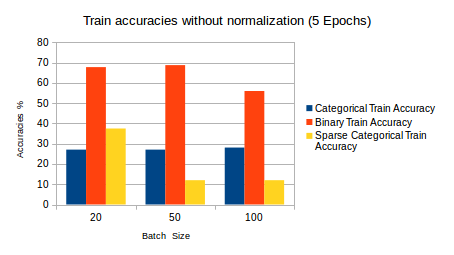
\includegraphics[scale=0.6]{trainCNNWONorm.png}
    \caption{Training accuracy results without normalization}
    \label{fig:trwo}
\end{figure}


\\

\begin{figure}[ht]
    \centering
    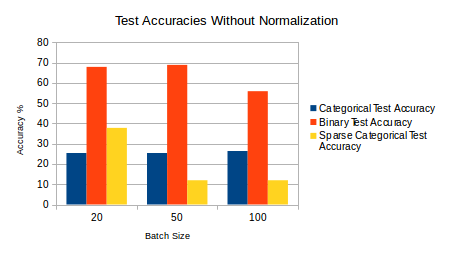
\includegraphics[scale=0.6]{TestCNNWONorm.png}
    \caption{Testing accuracy results without normalization}
    \label{fig:tewo}
\end{figure}

\\
\emph{With Normalization:}
\\
The range was changed from the original data to between 0 and 1 by dividing all the elements of the vectors by 255. This normalization technique was used because the vectors all had 0 as their minimum values and 255 as their maximum. This data was then input into a 3 layer CNN. The accuracy results were much better as compared to when non-normalized data was utilized. The highest accuracy for both training and testing sets found was 99.84 percent for training and 91.4 percent for testing which was achieved using binary cross entropy. The lowest training accuracy was found to be 77.71 percent while using sparse categorical cross entropy with batch size 100, while the lowest testing accuracy was found to be 80.99 percent while using batch size = 100. See Fig 3 and Fig 4 for the training and testing accuracy results by different loss functions for this experiment.
\\
\\
\begin{figure}[ht]
    \centering
    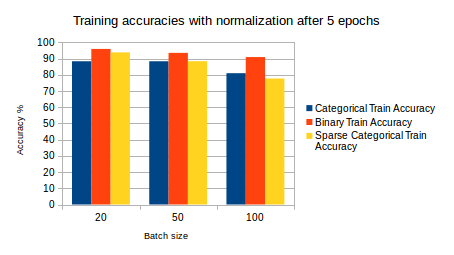
\includegraphics[scale=0.6]{TrainCNNNorm.png}
    \caption{Training accuracy results without normalization}
    \label{fig:my_label}
\end{figure}

\\

\\
\begin{figure}[ht]
    \centering
    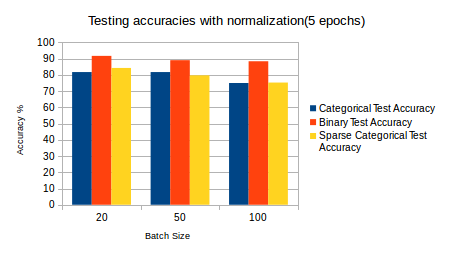
\includegraphics[scale=0.6]{testCNNNorm.png}
    \caption{Testing accuracy results without normalization}
    \label{fig:my_label}
\end{figure}

\\

\emph{Last Max-pooling layer added:}
\\
One experiment performed was to add the last max-pooling layer and check if the accuracies drop. The differences were relatively insignificant as the average accuracy drop was only around 2.1 percent for training and 1.3 percent for testing. See Fig 5 and Fig 6 for the training and testing accuracy results by different loss functions for this experiment.
\\

\\
\begin{figure}[ht]
    \centering
    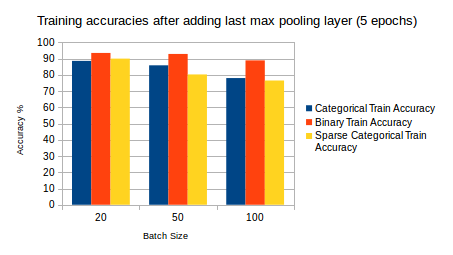
\includegraphics[scale=0.6]{TrainMaxPool.png}
    \caption{Training accuracy results with Max-Pooling added}
    \label{fig:my_label}
\end{figure}

\\

\\
\begin{figure}[ht]
    \centering
    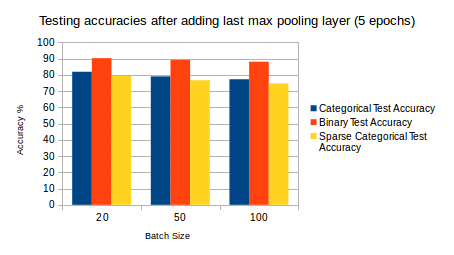
\includegraphics[scale=0.6]{testMaxPool.png}
    \caption{Testing accuracy results with Max-Pooling added}
    \label{fig:my_label}
\end{figure}

\\

\emph{Using ONNs:}
\\
After conducting experiments with CNN architectures, some experiments were also conducted with ONNs. This required concatenating all 10 seconds of data and flattening it into a 1280 length vector per sample. The highest accuracy found in this case was by the use of binary cross entropy and a batch size of 20 where the training accuracy was 95.6 percent and testing accuracy was 90.6 percent. One of the points to note in the comparison of the results from the CNNs and ONNs is that there is not a significant difference in the average training accuracy (approximately a 4.3 percent drop for ONNs), and an even smaller drop in the testing accuracy (approximately 2.2 percent). This could suggest that the CNN architecture used is too complex and caused some over-fitting. See Fig 7 and Fig 8 for the training and testing accuracy results by different loss functions for this experiment.

\\
\begin{figure}[ht]
    \centering
    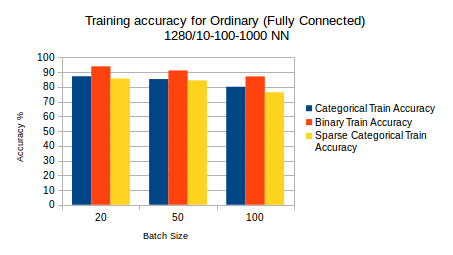
\includegraphics[scale=0.6]{TrainONN.png}
    \caption{Training accuracy results with ONNs}
    \label{fig:my_label}
\end{figure}

\\

\\
\begin{figure}[ht]
    \centering
    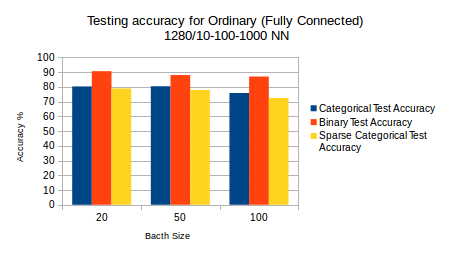
\includegraphics[scale=0.6]{TestONN.png}
    \caption{Testing accuracy results with ONNs}
    \label{fig:my_label}
\end{figure}

\\


\emph{Using Multiple Outputs:}
\\
A more ideal way to perform this kind of audio classification would be to use a single input embedding and obtain multiple outputs as a label. Therefore an experiment was also conducted using multi-output classification. However, the metric used is precision, as accuracy gives a false impression of good performance in this case. This is because accuracy doesn’t take into account false positives. The precision of each label was very low in this case (nearly 1.5 percent). 
\\
\\
\\
\\
\\
\\
\\
\\
\\
\\
\\
\\
\\
\\

\section{CONCLUSION}
\\
After observing the results, we can conclude that normalization of the features is essential in this kind of a classification task. We can also see that the batch size is an important factor in the performance of the model. Having a smaller batch size consistently gave more accurate results in these experiments. Another significant result in this experiment is that binary cross entropy as a loss function was very successful in gaining higher accuracies for the model. This can be explained by binary cross entropy dealing with each class as a separate classification task, where it decides whether the output is a “1” or a “0” for each category in a one-hot encoded vector. On the other hand, categorical cross entropies let the other categories affect the outcome of the probability of other classes in the classification task, as it uses a softmax activation function \cite{12}. Finally, the multi-label output classification performed poorly as there might not be enough training data to support the training of four simultaneous losses and outputs at the same time.

\begin{thebibliography}{13}


\bibitem{1}
    D. de Benito-Gorron et al, ”Exploring convolutional, recurrent, and hybrid deep neural networks for speech and music detection in a large audio dataset,” EURASIP Journal on Audio, Speech, and Music Processing, vol. 2019, (1), pp. 1-18, 2019.
\bibitem{2}
    S. Tseng et al, ”Multiple Instance Deep Learning for Weakly Supervised
    Small-Footprint Audio Event Detection,” 2017
\bibitem{3}
    A. Kumar, M. Khadkevich and C. Fugen, ”Knowledge transfer from
weakly labeled audio using convolutional neural network for sound
events and scenes,” in 2018, . DOI: 10.1109/ICASSP.2018.8462200.
\bibitem{4}
    A. Kumar and B. Raj, ”Audio Event Detection using Weakly Labeled
Data,” 2016.
\bibitem{5}
A. Shah et al, ”A Closer Look at Weak Label Learning for Audio
Events,” 2018.
\bibitem{6}
X. Xia et al, ”A Survey: Neural Network-Based Deep Learning for
Acoustic Event Detection,” Circuits, Systems, and Signal Processing,
2019.
\bibitem{7}
E. Cakir et al, ”Polyphonic sound event detection using multi label deep
neural networks,” in 2015, . DOI: 10.1109/IJCNN.2015.7280624.
\bibitem{8}
S. Adavanne and T. Virtanen, ”Sound event detection using weakly
labeled dataset with stacked convolutional and recurrent neural network,”
2017.
\bibitem{9}
Y. Zhang et al, ”Exploring Weakly Labeled Images for Video Object
Segmentation With Submodular Proposal Selection,” IEEE Transactions
on Image Processing, vol. 27, (9), pp. 4245-4259, 2018.
\bibitem{10}
Sound Event Detection and Time–Frequency Segmentation from Weakly
Labelled Data
\bibitem{11}
AudioSet: An ontology and human-labelled dataset for audio 
events
\bibitem{12}
K. Ghiasi-Shirazi, "Competitive Cross-Entropy Loss: A Study on Training Single-Layer Neural Networks for Solving Nonlinearly Separable Classification Problems," Neural Processing Letters, 2018.
\end{thebibliography}
\end{document}
